\documentclass{ximera}
      
\title{Pagerank Boxing in Sage}
      
\begin{document}
      
\begin{abstract}
      
This is a modified version of Google Pagerank used to rank boxers, based on their performance against each other.

\end{abstract}
      
\maketitle

Unless one is a student in an introductory linear algebra course, there is little to no reason to solve systems of equations or find eigenvectors by hand.  Even so, one could only be expected to do this for very small cases with nothing worth actually computing.  Thus we introduce a computer algebra system to do our heavy lifting for us.  The software we chose was Sage via sagecells.

\begin{example}
Suppose there are 5 boxers, $A,B,C,D, E$.  Boxer $A$ loses to $B$ who then loses to $C$.  Then $E$ fights $B$ to a draw, and $D$ also fights $A$ and wins.  Afterwards $E$ and $B$ have a rematch and $E$ wins:
 
\begin{figure}[h]
\centering
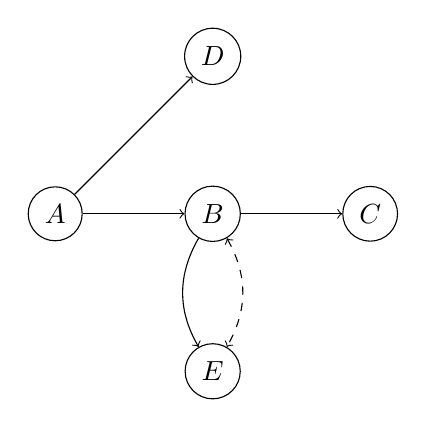
\begin{tikzpicture}
\node[shape=circle, draw, radius=0.25] (A) at (0,0){$A$};
\node[shape=circle, draw, radius=0.25] (B) at (2,0){$B$};
\node[shape=circle, draw, radius=0.25](C) at (4,0){$C$};
\node[shape=circle, draw, radius=0.25] (D) at (2,2){$D$};
\node[shape=circle, draw, radius=0.25] (E) at (2,-2){$E$};


\draw[->](A) -- (B);
\draw[->](B) -- (C);
\draw[->](A) -- (D);
\draw[<->, dashed](B) to [bend left] (E);
\draw[->](B) to [bend right](E);

\end{tikzpicture}
    \caption{A more complex boxing network}
    \label{complex}

\end{figure}

 
 What would be the respective ranking of these boxers? Would $D$ be ranked the same as $C$ as they are both undefeated?  How does $E$ compare to everyone?
 
 \end{example}
 
 To evaluate this, using the modified pagerank described \link[here]{https://drive.google.com/open?id=0B9tqGFTzh_9uczlkQkIwb2hqNmc}, we consider the following code:
 
 \begin{sageCell}
 #We first create the raw data matrix
listsize=5 # This determines the number of boxers being compared
rawdata=matrix(QQ,listsize,listsize); #This creates a zero square matrix of the appropriate size, the entries of this matrix are allowed to be rational.

#We then input the win/loss data into the matrix, the += command increments the appropriate entry by the given amount.  If boxer i loses to boxer j, we encode that by rawdata[i,j]+=1.  If Boxer i and j tie, we encode that by rawdata[i,j]+=1/2 and rawdata[j,i]+=1/2
#Recall that in Sage, arrays are enumerated starting at 0, so the first entry is the 0th entry, rather than the 1st.

rawdata[0,1]+=1
rawdata[0,3]+=1 #These encode the losses suffered by A
rawdata[1,2]+=1
rawdata[1,4]+=1/2
rawdata[1,4]+=1 #These encode the losses and tie by boxer B
# Boxers C and D didnot suffer ties or losses and so there are no entries for those rows
rawdata[4,1]+=1/2 #This encodes the tie by E to C

#The following lines encodes an adjacency matrix adj for the underlying unweighted, undirected graph, should there be some interest in it's structure.
adj=matrix(QQ,listsize,listsize);

for i in range(listsize):
    for j in range (listsize):
        if rawdata[i,j]!=0:
            adj[i,j]=1
            adj[j,i]=1

            
            
#The following lines encodes an adjacency matrix adj for the underlying unweighted, directed graph, should there be some interest in it's structure.

dij=matrix(QQ,listsize,listsize);

for i in range(listsize):
    for j in range (listsize):
        if rawdata[i,j]!=0:
            dij[i,j]=1


#The following lines creates the normalized data matrix, where multiple-fights are normalized
normal=matrix(QQ,listsize,listsize)

for i in range(listsize):
    for j in range (listsize):
        if rawdata[i,j]+rawdata[j,i]!=0:
            normal[i,j]=rawdata[i,j]/(rawdata[i,j]+rawdata[j,i]) 

#If you wish to the normal matrix, comment out the first line under this if listsize<20.  Otherwise, comment out the following 2 lines
#normal #Uncomment this line to see normal if listsize<20
#for i in range (listsize): #Uncomment this and the following line if listsize >=20.
#    print normal.rows()[i]


            
#We then create the stochastic data matrix:
stoch=matrix(QQ,listsize,listsize)
    
for i in range(listsize):
    rowsum=0
    for j in range(listsize):
        rowsum=rowsum+normal[i,j]
    if rowsum!=0:
        for k in range(listsize):
            stoch[i,k]=normal[i,k]/rowsum #This stochasticizes rows for non-undefeated fighters.
    else:
        for l in range(listsize):
            stoch[i,l]=1/listsize #This creates the rows for undefeated fighters and allows stoch to be a true markov matrix

#If you wish to the stoch matrix, comment out the first line under this if listsize<20.  Otherwise, comment out the following 2 lines
#stoch #Uncomment this line to see normal if listsize<20
#for i in range (listsize): #Uncomment this and the following line if listsize >=20.
#    print stoch.rows()[i]

#We then create the positive stochastic matrix M

J=matrix(QQ,listsize,listsize);

for i in range(listsize):
    for j in range(listsize):
        J[i,j]=1 #This creates a square matrix where each value is 1
p=15/100 #The damping factor p
M=(1-p)*stoch+p*(1/listsize)*J #The final matrix M

#If you wish to the M matrix, comment out the first line under this if listsize<20.  Otherwise, comment out the following 2 lines
#M #Uncomment this line to see normal if listsize<20
#for i in range (listsize): #Uncomment this and the following line if listsize >=20.
#    print M.rows()[i]


#The following lines identifies which eigenvalue/vector pair has eigenvalue 1
sizespec=len(M.eigenvectors_left())

stable=0

for i in range(sizespec):
    if M.eigenvectors_left()[i][0]==1:
        stable=i

        
#We then list the entries of the appropriate eigenvector in order, mutiplying by 1.0 gives a decimal approximation for easier comparison
        
for i in range(len(M.eigenvectors_left()[stable][1][0])):
    show(M.eigenvectors_left()[stable][1][0][i]*1.0)
    

#We then display the digraph based on the normalized data matrix so as to visualize the win/loss relationship between boxers    
G = DiGraph(normal)
H = G.plot(color_by_label=True)
H.show()\end{sageCell}

















\end{document}
